\documentclass[a4paper,12pt]{article}
\usepackage[colorlinks,linkcolor=black,urlcolor=black]{hyperref}
\usepackage{float}
\usepackage[table,xcdraw]{xcolor}
\usepackage{mathrsfs}
\usepackage{pdfpages}
\usepackage{enumerate}
\usepackage{amsmath}
\usepackage{setspace}
\usepackage{booktabs}
\usepackage{colortbl}
\usepackage{titlesec}
\usepackage{amssymb}
\usepackage{csquotes}
\usepackage{graphicx}
\usepackage{subfigure}
\usepackage{siunitx}
\usepackage{wrapfig}
\usepackage{geometry}
\usepackage{indentfirst}
\usepackage{multirow} 
\usepackage{listings}

\setlength{\parindent}{2em}
\renewcommand{\mkbegdispquote}[2]{\itshape}
\renewcommand{\baselinestretch}{1.15}
\usepackage[greek,english]{babel} 
\geometry{left=2.2cm,right=2.2cm,top=1.7cm,bottom=1.7cm}


\begin{document}

\begin{titlepage}

\begin{figure}[!htbp]
\center

\includegraphics[scale=0.7,width=12cm]{ji_logo.png}
\end{figure}

\noindent\rule[0.25\baselineskip]{\textwidth}{1pt}

\begin{center}

\Large{\bfseries  VV557 Methods of Applied Mathematics II}

\vspace{2cm}

\Large{\bfseries  Term Project:}\\
\Huge{{\bfseries A Short Introduction to Boundary Element Method}}

\vspace{5cm}

\large{\textbf{Written by}}\\ 

\begin{tabular}{l l}
Zhou Zhanpeng & 518021910594\\
\end{tabular}

\textbf{Instructed by}\\
Dr. Horst Hohberger\\

\vspace{3cm}


{\bfseries \today}\\

\vspace{0.5cm}

\fbox{
  \parbox{14cm}{
    \begin{center}
\small{University of Michigan - Shanghai Jiao Tong University Joint Institute  \\
(UM-SJTU JI)  \\
800 Dongchuan Road, Shanghai, China 200240 }
    \end{center}
  }
}

\end{center}

\end{titlepage}

\begin{abstract}
After nearly 40 years of research and development, the boundary element method has become an accurate and efficient engineering numerical analysis method to solve boundary value problem in such fields as mathematics and physics. Aiming to give a short introduction to BEM, in this paper, we will explore the internal principle and performance of boundary element method by solving a simple Dirichlet problem, discuss boundary element method using Green function, and then investigate further on BEM applied mixed boundary value problem.
\end{abstract}

\tableofcontents

\newpage

\section{Introduction}
The boundary element method is a relatively new numerical method developed after the finite element method. With nearly 40 years of research and development, the boundary element method has become an accurate and efficient engineering numerical analysis method in such fields as mathematics and physics. Different from the basic idea of finite element method to divide elements in the continuum domain, boundary element method only divides elements on the boundary of the domain and approximates the boundary condition with the function satisfying the governing equation. Therefore, compared with the finite element method, BEM has the advantages of fewer elements and simpler calculations. 

\par In this paper, we are aimed to give a short introduction to BEM. Therefore, in the following sections, we will first explore the internal principle and performance of BEM by solving a simple Dirichlet problem, then discuss the performance of BEM using Green function, and finally investigate further on BEM applied to mixed boundary value problem. 

\section{Dirichlet Problem for the Laplace Equation On The Half-disk}
To explain the principle of BEM  more clearly, we will focus on a simple Dirichlet problem governed by the two-dimensional Laplace's equation on the half-disk in the following several sections. Therefore, it is convenient for us to define the problem in advance.

\par Thus, we set
\begin{equation}
\Omega = \{ (x_1,x_2) \in R^2: x_1^2 + x_2^2 < 1, x_2 > 0 \}
\end{equation}

\par Also,
\begin{align}
&- \Delta u = 0 \ {\rm on}\   \Omega & \begin{aligned}
&u(x_1,x_2)|_{x_1^2 + x_2^2} = 1 \\ &u(x_1,0) = 0  \ {\rm for} \ -1 < x_1 < 1
\end{aligned}
\end{align} 

\section{The Analytic Solution to the Dirichlet Problem}
Before we really get started with BEM, we need to have a basic idea of the solution to the Dirichlet problem. Therefore, we will first use method of images[1] to find the green function and then find the analytic solution to the Dirichlet problem. 

\par First, according to method of images[1], we could find our images as shown in figure 1.
\begin{figure}[H]
\centering
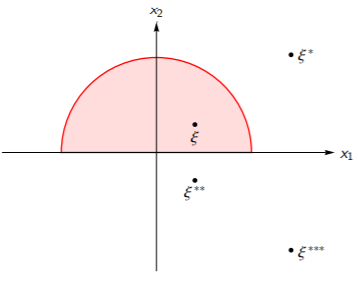
\includegraphics[scale=0.7]{1.png}
\caption{Images of the half-disk problem[1]}
\end{figure}
\noindent Supposing $\xi = (\xi_1, \xi_2) \in \Omega$, then
\begin{equation*}
\begin{aligned}
&\xi^* = \frac{\xi}{|\xi|^2} = \frac{1}{|\xi|^2}(\xi_1, \xi_2)\\
&\xi^{**} = (\xi_1 , - \xi_2) \\
&\xi^{***} = \frac{1}{|\xi|^2}(\xi_1, -\xi_2)
\end{aligned}
\end{equation*}
Also, it is known that the fundamental solution to $-\Delta E = \delta(x - \xi)$ is

\begin{equation*}
\begin{aligned}
E(x;\xi) =  - \frac{1}{2\pi} \ln|x - \xi| \ \ [1]
\end{aligned}
\end{equation*}
Thus, it is not hard for us to construct the green function of this problem 

\begin{equation*}
\begin{aligned}
g(x;\xi) &= E(x;\xi) - E(x;\xi^*) - E(x;\xi^{**}) + E(x;\xi^{***})\\
&=- \frac{1}{2\pi} \ln|x - \xi| + \frac{1}{2\pi} \ln|x - \xi^*| + \frac{1}{2\pi} \ln|x - \xi^{**}| - \frac{1}{2\pi} \ln|x - \xi^{***}|
\end{aligned}
\end{equation*}
which obviously satisfy the boundary conditions that 

\begin{equation*}
\begin{aligned}
&g(x,y)|_{x_1^2 + x_2^2} = 0 & g(x_1,0) = 0 \ {\rm for} \  -1 < x_1 <1
\end{aligned}
\end{equation*}
Then, based on the solution formula for Epllitic problem[1], the solution formula for our specific problem can be found as
\begin{equation*}
\begin{aligned}
u(\varrho, \vartheta) &= - \int_{0}^{\pi} \frac{\partial }{\partial r}g(r, \theta;\varrho, \vartheta)|_{r= 1} d \theta \ \ [1]
\end{aligned}
\end{equation*}
However, due to our solution formula is defined in polar coordinates, it is necessary to transform the green function into polar coordinates

\begin{equation*}
\begin{aligned}
&\xi  =(\xi_1,\xi_2) = (\varrho \cos\vartheta, \varrho\sin\vartheta)\\
&x = (x_1,x_2) = (r\cos\theta,r\sin\theta)
\end{aligned}
\end{equation*}
Now, we can calculate $\frac{\partial g}{\partial r}$. For example, 
$$
\frac{1}{2\pi} \ln|x - \xi| = \frac{1}{4\pi}\ln((r\cos\theta - \varrho\cos\vartheta)^2+ (r\sin\theta - \varrho\sin\vartheta)^2)
$$ 
Then 

\begin{equation*}
\begin{aligned}
\frac{\partial \frac{1}{2\pi} \ln|x - \xi|}{\partial r} &= \frac{\partial \frac{1}{4\pi}\ln((r\cos\theta - \varrho\cos\vartheta)^2+ (r\sin\theta - \varrho\sin\vartheta)^2)}{\partial r}\\
&= \frac{1}{2\pi} \frac{r - \varrho(\cos(\theta - \vartheta))}{r^2 - 2\varrho r(\cos(\theta - \vartheta)) + \varrho^2}
\end{aligned}
\end{equation*}
Similarly, it is easy for us to find

\begin{equation*}
\begin{aligned}
\frac{\partial  \frac{1}{2\pi} \ln|x - \xi^*|}{ \partial r} = \frac{1}{2\pi} \frac{\varrho^2r - \varrho(\cos(\theta - \vartheta))}{\varrho^2r^2 - 2\varrho r(\cos(\theta - \vartheta)) + 1}
\end{aligned}
\end{equation*}
And

\begin{equation*}
\begin{aligned}
\frac{\partial  \frac{1}{2\pi} \ln|x - \xi^{**}|}{ \partial r} = \frac{1}{2\pi} \frac{r - \varrho(\cos(\theta + \vartheta))}{r^2 - 2\varrho r(\cos(\theta + \vartheta)) + \varrho^2}
\end{aligned}
\end{equation*}
Also,

\begin{equation*}
\begin{aligned}
\frac{\partial  \frac{1}{2\pi} \ln|x - \xi^{***}|}{ \partial r} = \frac{1}{2\pi} \frac{\varrho^2r - \varrho(\cos(\theta + \vartheta))}{\varrho^2r^2 - 2\varrho r(\cos(\theta + \vartheta)) + 1}
\end{aligned}
\end{equation*}
Finally, the analytic solution to this problem could be found:

\begin{equation*}
\begin{aligned}
u(\varrho, \vartheta) &=- \int_{0}^{\pi} \frac{\partial}{\partial r}g(r, \theta;\varrho, \vartheta)|_{r= 1} d\theta\\
&=\frac{\varrho^2 -1}{2\pi}\int_{0}^{\pi}( \frac{1}{\varrho^2 + 1 - 2\varrho\cos(\theta + \vartheta)} - \frac{1}{\varrho^2 + 1 - 2\varrho\cos(\theta - \vartheta)}) d\theta \\
&= \left(\frac{1}{\pi}\arctan(\frac{1 + \varrho}{1 - \varrho}\tan\frac{\theta - \vartheta}{2}) -  \frac{1}{\pi}\arctan(\frac{1 + \varrho}{1 - \varrho}\tan\frac{\theta + \vartheta}{2})\right) |_{0}^{\pi} -1\\
&= \frac{2}{\pi}\arctan(\frac{1 + \varrho}{1 - \varrho}\tan\frac{\vartheta}{2}) +  \frac{2}{\pi}\arctan(\frac{1 + \varrho}{1 - \varrho}\cot\frac{\vartheta}{2}) -1
\end{aligned}
\end{equation*}

Just to make the solution to this problem more intuitive, using Mathematica,  a scientific computational tool, we could plot the solution on a three-dimensional plane as shown in figure 2. 

\begin{figure}[H]
\centering
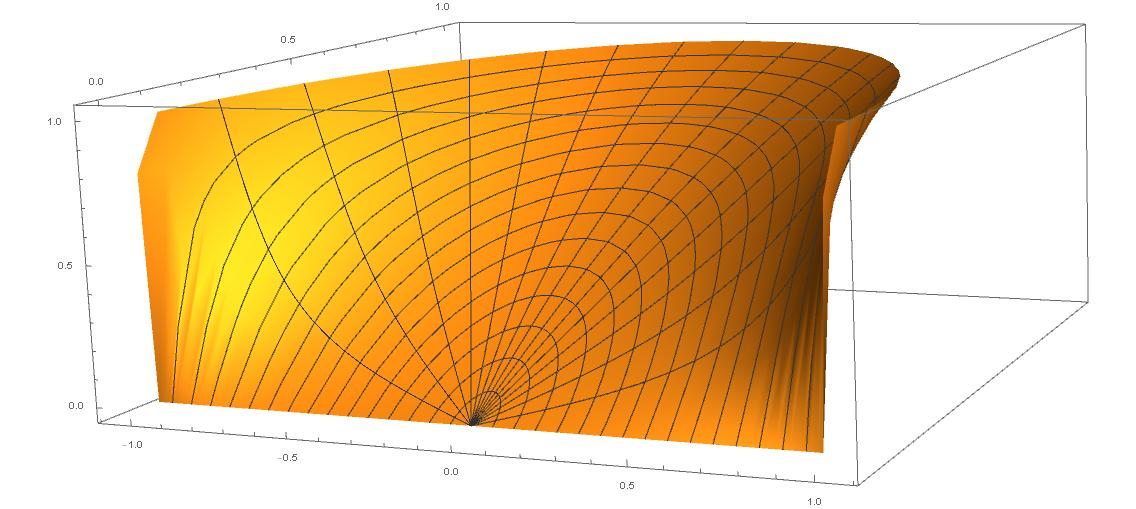
\includegraphics[scale=0.3]{analytic.jpg}
\caption{The analytic solution to the Dirichlet problem}
\end{figure}

\section{Boundary Element Methods}
However, how does BEM actually work? In this section, we will first start from the derivation of BEM, then apply BEM to the Dirichlet problem which we defined earlier and compare the obtained numerical solution with analytic solution to see how BEM performs.
\subsection{Boundary Integral solution}
\par To explain the internal principle of BEM, we should start from the basis of BEM, the boundary integral solution[2].
\par Supposing $\phi_1$ and $\phi_2$ are two solution of Eq. (2) in the region $\Omega$, then, it is known that

\begin{equation}
\int_{\partial \Omega} (\phi_2 \frac{\partial \phi_1}{\partial n} - \phi_1 \frac{\partial \phi_2}{\partial n}) ds = 0
\end{equation}
which is called reciprocal relation[2] that can be easily derived from divergence theorem. 

\par If we take $\phi_1 = E(x;\xi)$, the fundamental solution to the Eq. (2) and $\phi_2 = u$, where $u$ is the required solution[2] of the boundary value problem. Then, the reciprocal relation[2] can be written as

\begin{equation}
\int_{\partial \Omega} [u(x)\frac{\partial E(x_;\xi)}{\partial n} - E(x;\xi) \frac{\partial u(x)}{\partial n}] ds = 0 \ \ [2]
\end{equation}
where $\xi \notin \Omega$, due to $E(x;\xi)$ is not well-defined on the point $\xi$ [2]. 

\par However, we can still make $\xi$ in the interior of $\Omega$ as long as we modify the boundary as $\partial \Omega \cup \partial \Omega_{\varepsilon}$ where $\Omega_{\varepsilon}$ is a circle of center $\xi$ and radius $\varepsilon$ [2]. Thus, we can rewrite Eq. (4) as

\begin{equation}
\int_{\partial \Omega \cup \partial \Omega_{\varepsilon}} [u(x)\frac{\partial E(x_;\xi)}{\partial n} - E(x;\xi) \frac{\partial u(x)}{\partial n}] ds = 0 \ \ [2]
\end{equation}
which can be also written as
\begin{equation}
\int_{\partial \Omega } [u(x)\frac{\partial E(x_;\xi)}{\partial n} - E(x;\xi) \frac{\partial u(x)}{\partial n}] ds = -\int_{\partial \Omega_{\varepsilon} } [u(x)\frac{\partial E(x_;\xi)}{\partial n} - E(x;\xi) \frac{\partial u(x)}{\partial n}] ds \ \ [2]
\end{equation}

\par if we use polar coordinates instead, the coordinates should be defined as
\begin{equation}
\begin{aligned}
x_1 - \xi_1 = r \cos \theta \\
x_2 - \xi_2 = r \sin\theta
\end{aligned}
\end{equation}
Then, it is easy for us to obtain the fundamental solution and its normal derivative in polar coordinates
\begin{equation}
\begin{aligned}
& E (x;\xi) = \frac{1}{2\pi} \ln (r)
& \frac{\partial E}{\partial n} = \frac{n_{x_1} \cos\theta + n_{x_2} \sin\theta}{2\pi r} \ \ [2]
\end{aligned}
\end{equation}
Also, we know the Taylor's series of $u$ about the point $\xi$ is
\begin{equation*}
u = \sum_{m = 0}^{\infty}\sum_{k = 0}^{m } (\frac{\partial u}{\partial x_1^{k} \partial x_2^{m - k}})|_{(x_1,x_2) = (\xi_1,\xi_2)} \frac{(x_1- \xi_1)^k(x_2 - \xi_2)^{m - k}}{k!( m - k)!}  \ \ [2]
\end{equation*}
Then, for all the points on the circle $\partial \Omega_{\varepsilon}$, with polar coordinates, $u$ can be also written as 
\begin{equation}
u = \sum_{m = 0}^{\infty}\sum_{k = 0}^{m } (\frac{\partial u}{\partial x_1^{k} \partial x_2^{m - k}})|_{(x_1,x_2) = (\xi_1,\xi_2)} \frac{\varepsilon^m \cos^k \theta \sin^{m - k}\theta}{k!( m - k)!} \ \ [2]
\end{equation}
Similarly, we can get
\begin{equation}
\frac{\partial u}{\partial n} = \sum_{m = 0}^{\infty}\sum_{k = 0}^{m } (\frac{\partial}{\partial x_1^{k} \partial x_2^{m - k}}\frac{\partial u}{\partial n})|_{(x_1,x_2) = (\xi_1,\xi_2)} \frac{\varepsilon^m \cos^k \theta \sin^{m - k}\theta}{k!( m - k)!} \ \ [2]
\end{equation}

With Eq. (8), Eq. (9), Eq. (10) and knowing $d s = \varepsilon d \theta $[2], we can then rewrite the right hand side of Eq. (6) as
\begin{equation}
\begin{aligned}
&\int_{\partial \Omega_{\varepsilon} } u(x)\frac{\partial E(x_;\xi)}{\partial n} d s \\
&= - u(\xi) - \frac{1}{2\pi} \sum_{m = 1}^{\infty}\sum_{k = 0}^{m } (\frac{\partial u}{\partial x_1^{k} \partial x_2^{m - k}})|_{(x_1,x_2) = (\xi_1,\xi_2)} \frac{\varepsilon^m }{k!( m - k)!}\int_{0}^{2\pi} \cos^k \theta \sin^{m - k}\theta \theta d\theta \ \ [2]
\end{aligned}
\end{equation}
which will be approximately equal to $ - u(\xi)$ as $\varepsilon \to 0^+$ [2]. 
\par Also, 
\begin{equation}
\begin{aligned}
&\int_{\partial \Omega_{\varepsilon} } E(x)\frac{\partial u(x_;\xi)}{\partial n} d s \\
&= \frac{1}{2\pi} \sum_{m = 0}^{\infty}\sum_{k = 0}^{m } (\frac{\partial }{\partial x_1^{k} \partial x_2^{m - k}}(\frac{\partial u}{\partial n}))|_{(x_1,x_2) = (\xi_1,\xi_2)} \frac{\varepsilon^{m+1} \ln(\varepsilon) }{k!( m - k)!}\int_{0}^{2\pi} \cos^k \theta \sin^{m - k}\theta \theta d\theta \ \ [2]
\end{aligned}
\end{equation}
which will be approximately equal to $0$ as $\varepsilon \to 0^{+}$ [2]. 

\par Therefore, as $\varepsilon \to 0^{+}$ Eq. (6) yields

\begin{equation}
u(\xi) = \int_{\partial \Omega } [u(x)\frac{\partial E(x_;\xi)}{\partial n} - E(x;\xi) \frac{\partial u(x)}{\partial n}] ds \ \ [2]
\end{equation}

\par However, so far, $\xi$ can be only be the points inside the $\Omega$.  If $\xi$ are exactly at the boundary, $\partial \Omega_{\varepsilon}$ should be modified as a semicircle [2]. Correspondingly, for those $\xi$ at the boundary, our Eq. (13) should be modified as 
\begin{equation}
\frac{1}{2}u(\xi) = \int_{\partial \Omega } [u(x)\frac{\partial E(x_;\xi)}{\partial n} - E(x;\xi) \frac{\partial u(x)}{\partial n}] ds \ \ [2]
\end{equation}
What's more, for those the points are even not contained in $\Omega$, it is obvious that 
\begin{equation}
\int_{\partial \Omega } [u(x)\frac{\partial E(x_;\xi)}{\partial n} - E(x;\xi) \frac{\partial u(x)}{\partial n}] ds = 0 \ \ [2]
\end{equation}
Then, for convenience, we combine Eq. (13), Eq. (14), Eq. (15) together as a single equation which is
\begin{equation}
\lambda(\xi)u(\xi) = \int_{\partial \Omega } [u(x)\frac{\partial E(x_;\xi)}{\partial n} - E(x;\xi) \frac{\partial u(x)}{\partial n}] ds  \ \ [2]
\end{equation}
where $\lambda (\xi)$ is defined as
\begin{equation}
\lambda(\xi) = \left\{
\begin{aligned}
&0 &{\rm if} \xi \notin \Omega\\
&\frac{1}{2} &{\rm if} ]\xi \in \partial\Omega\\
&1 &{\rm if} \xi \in \Omega \cap \xi \notin  \xi \partial\Omega\\
\end{aligned} 
\right. \ \ [2]
\end{equation}

As shown above, the combined mathematical formula is just the boundary integral solution[2].

\subsection{Boundary Element Method}
We have shown the basis of boundary element method, the boundary integral solution, in the last section. Now, we will introduce a simple procedure of implementing BEM to show how BEM Works.

\subsubsection*{Step 1: Discretize Boundary $C$ }
First, we should divide the boundary into a few elements. For simplicity, we define $C = \partial \Omega$ [2], then, take arbitrary points on the boundary, as illustrated in the figure 3, $x^{k} \in C$ where $k = 1,2, \cdots N$, to divides $C$ into the $N$ small line segments, $C^{1}, C^2, \cdots, C^{N}$[2].

\begin{figure}[H]
 \centering
 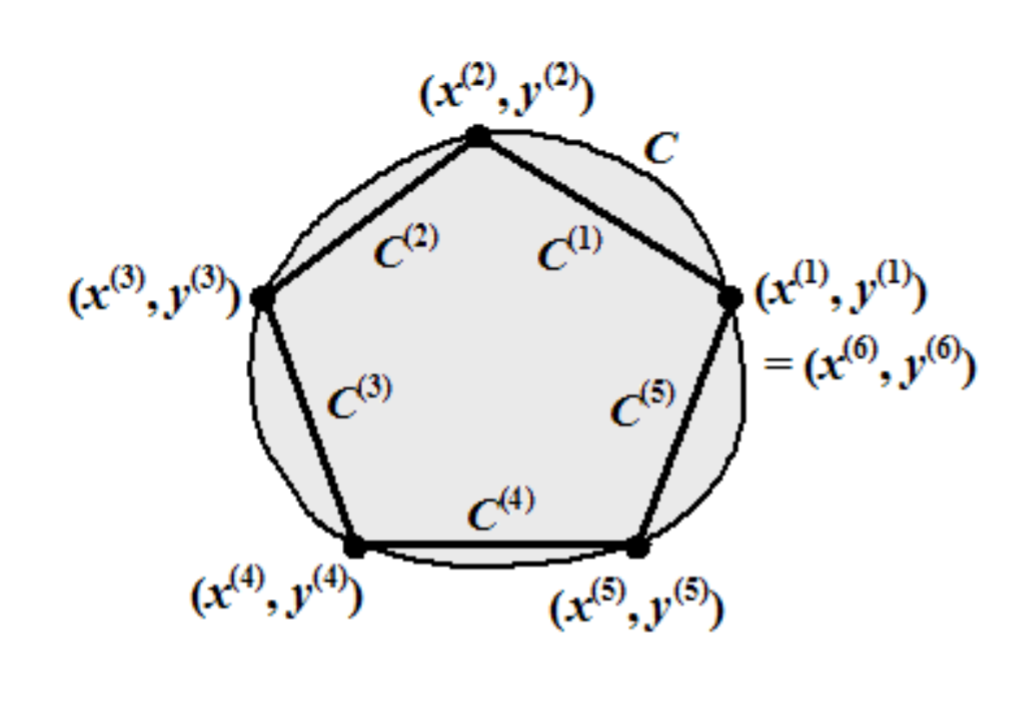
\includegraphics[scale=0.5]{2.png}
 \caption{Discretize the boundary $C$ [2]}
 \end{figure}
  
Based on that, we can approximate the boundary $C$ as the combination of all the line segments. That is
\begin{equation}
C \approx C^1 \cup C^2 \cup \cdots \cup C^{N-1} \cup C^N \ \ [2]
\end{equation}

\subsubsection*{Step 2: Approximate Boundary Integral Solution}

\par Then, we will make an approximation of $u$ and $\frac{\partial u}{\partial n}$ on each line segment $C^k$. If the line segments are small enough, it is sufficient for us to take the $u$ and $\frac{\partial u}{\partial n}$ at the mid point of the segment as a good approximation to the real value of $u$ and $\frac{\partial u}{\partial n}$ at each point of the line segment[2]. Thus, we use following approximations,

\begin{equation}
\begin{aligned}
&u \approx \bar{u}^k & \frac{\partial u}{\partial n} \approx \bar{p}^k \ {\rm for }\ (x_1,x_2) \in C^k (k = 1,2,\cdots, N) \ \ [2]
\end{aligned}
\end{equation}
where $\bar{u}^k$ and $\bar{p}^k$ are the values of $u$ and $\frac{\partial u}{\partial n}$ at the midpoint of $C^k$. 

\par Then based on our approximations, the boundary integral solution[2] can be written as
\begin{equation}
\lambda(\xi) u(\xi) \approx  \sum_{k = 1}^{N} (\bar{u}^{k} F_{2}^{k}(\xi) - \bar{p}^k F_{1}^k(\xi)) \ \ [2]
\end{equation}
where
\begin{equation}
\begin{aligned}
&F_{1}^{k}(\xi) = \int_{C^k} E(x;\xi) d s\\
&F_{2}^{k}(\xi) = \int_{C^k} \frac{\partial}{\partial n} E(x;\xi) d s
\end{aligned} \ \ [2]
\end{equation}

\par Now, we have derived the boundary element solution, which is just Eq. (20) and in most cases, $F_1^k$ and $F_2^k$ are easily calculated. However, we are not done, some unknown constants in the Eq. (20) still need to be found. 

\subsubsection*{Step 3: Calculate Unknown Constants}
Due to constrain of the boundary condition, either $\bar{u}^k$ or $\bar{p}^k$ is known, therefore, there are $N$ unknown constants in our boundary element solution. Thus, we should construct a linear system with $N$ independent equations to solve all the $N$ unknown constants. 
\par Here, by substituting the midpoints of $C^1, C^2, \cdots, C^N$ into the boundary element solution, we obtain the linear system
\begin{equation}
\frac{1}{2} \bar{u}^m = \sum_{k = 1}^m (\bar{u}^k F_2^k(\bar{x_1}^m,\bar{x_2}^m) - \bar{p}^m F_1^k(\bar{x_1}^m,\bar{x_2}^m))\  {\rm for } \ m = 1,2,\cdots N \ \ [2]
\end{equation} 
where $(\bar{x_1}^m,\bar{x_2}^m)$ is the midpoint of $C^m$. 

\par However, to simplify our calculations, we can also rewrite Eq. (22) as
\begin{equation}
\sum_{k =1}^{N} a^{mk} z^k = \sum_{k =1}^{N} b^{mk} \  {\rm for } \ m = 1,2,\cdots N \ \ [2]
\end{equation}
where $a^{mk},b^{mk},z^{k}$ are 
\begin{equation}
\begin{aligned}
&a^{mk} = \left\{\begin{aligned} &-F_1^k(\bar{x_1}^m,\bar{x_2}^m) &{\rm if \ u \  is \ specified \ over \ C^k}\\& F_2^k(\bar{x_1}^m,\bar{x_2}^m) - \frac{1}{2} \delta^{mk} &{\rm if \ \frac{\partial u}{\partial n} \  is \ specified \ over \ C^k} \end{aligned}\right.\\
&b^{mk} = \left\{\begin{aligned} &\bar{u}^k(-F_2^k(\bar{x_1}^m,\bar{x_2}^m) + \frac{1}{2}\delta^{mk}) &{\rm if \ u \  is \ specified \ over \ C^k}\\& \bar{p}^kF_1^k(\bar{x_1}^m,\bar{x_2}^m) &{\rm if \ \frac{\partial u}{\partial n} \  is \ specified \ over \ C^k} \end{aligned}\right.\\
&\delta^{mk} = \left\{\begin{aligned} &0 &{\rm if \ m \neq k}\\& 1 &{\rm if \ m = k} \end{aligned}\right.\\
&z^{k} = \left\{\begin{aligned} &\bar{p}^k &{\rm if \ u \  is \ specified \ over \ C^k}\\& \bar{u}^k &{\rm if \ \frac{\partial u}{\partial n} \  is \ specified \ over \ C^k} \end{aligned}\right.\\
\end{aligned} \ \ [2]
\end{equation}
\subsubsection*{Summary}
Applying BEM to solve a boundary value problem, we should first divide the boundary into many line segments and use Eq. (21) to solve both values of $F_1$ and $F_2$ on each line segment. Then, we should solve the linear system Eq. (23,24) to get all the unknown constants in the boundary element solution. Finally, we can plug all the calculation results into Eq. (20) to obtain the numerical solution to the BVP. 

\subsection{Boundary Element Solution of Pre-defined Problem and Comparison with Analytic Solution}
In previous section, we have talked about the detailed principle and derivation of BEM. However, someone may ask, how does BEM perform in reality. In this section, we will apply BEM to the pre-defined problem, the Dirichlet problem governed by the two-dimensional Laplace's equation on the half-disk, and compare the numerical solution with analytic solution which have been obtained in previous section. 

\par Following the steps in the last section, we firstly divide the semi-circle into $120$ line segments as roughly shown in figure 4.
\begin{figure}[H]
\centering
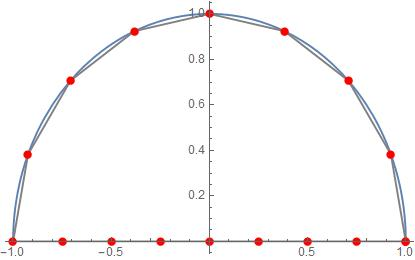
\includegraphics[scale=0.55]{segments.jpg}
\caption{Rough idea to divide the boundary of half-disk}
\end{figure}

Then, we use Mathematica to calculate both values of $F_1$ and $F_2$ on each line segment and all the unknown constants (detailed code are attached in \textbf{Appendix}). Finally, we obtain the numerical solution (with $120$ constants elements) and plot the solution in 3D-plane as shown in the figure 5 below.
\begin{figure}[H]
\centering
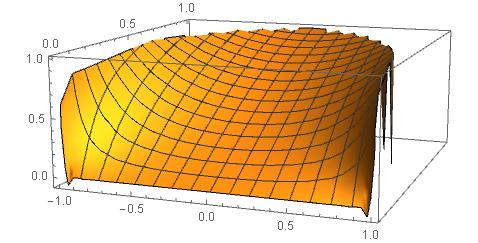
\includegraphics[scale=0.6]{BEM.jpg}
\caption{Boundary element solution to pre-defined problem}
\end{figure}

\par Comparing our plot of the numerical solution (figure 5) with previous plot of analytic solution (Figure 1), it is obvious that although both plots are almost same, the plot of numerical solution at the boundary is not as smooth as that of analytic solution. However, just drawing rough statements from visual observation is not sufficient, we will compare the two solution into details.

In the table 1 below, the numerical value of $u$ (as calculated by the boundary element procedure with $60$ and $120$ constant elements) at an input interior point ($\xi_1, \xi_2$) is compared with the exact solution.   

\begin{table}[H]
\centering
\begin{tabular}{@{}cccc@{}}
\toprule
   $(\xi_1,\xi_2)$         & 60 Elements & 120 Elements & Exact    \\ \midrule
(0.10,0.20) & 0.253818     & 0.253738      & 0.253707 \\
(0.10,0.30) & 0.374508    & 0.374381     & 0.374334 \\
(0.10,0.40) & 0.488517     & 0.488345     & 0.488284 \\
(0.50,0.20) & 0.326754     & 0.326665      & 0.326623 \\
(0.50,0.30) & 0.469958     & 0.469776      & 0.469708 \\
(0.50,0.40) & 0.595803     & 0.595548      & 0.595458 \\
(0.90,0.20) & 0.773119    & 0.771894      & 0.771599 \\
(0.90,0.30) & 0.896111     & 0.895153      & 0.894863 \\
(0.90,0.40) & 0.977072     & 0.976404      & 0.976138 \\ \bottomrule
\end{tabular}
\caption{Comparing numerical value of $u$ with exact value at given interior points}
\label{tab:my-table}
\end{table}
\par From the table, it is clear that there is a significant improvement in the accuracy of the numerical results when the number of constants elements increases from $60$ to $120$. And when we use $120$ constant elements, the numerical values has almost same number with the exact values. 

\par We also examine the accuracy of the numerical value of $u$ (as calculated by the boundary element procedure with $120$ constant elements) at the interior point ($0.1, a$) as $a$ approaching 1 from $0.95$. The results are listed in table 2 below. 

\begin{table}[H]
\centering
\begin{tabular}{@{}cccccc@{}}
\toprule
Error       & 0.95       & 0.96        & 0.97        & 0.98        & 0.99         \\ \midrule
120 Elements & 0.000102288 & 0.000102576 & 0.000103059 & 0.00010473 & 0.000112379 \\ \bottomrule
\end{tabular}
\caption{Errors of numerical solution with $60$ constant elements at some given interior points}
\label{tab:my-table}
\end{table}
\par From the table 2, it is clear that as interior points approaching to boundary, the errors get larger and larger. The results coincide with the well-known fact that the accuracy of a boundary element solution may deteriorate significantly at a point whose distance from the boundary is very small compared with the lengths of nearby boundary elements[2]. 

\par However, we only talked about interior points so far. What about the points which are exactly on the boundary? Will $u$ at boundary points differ a lot with exact value? Here, we plot $u$ (with $120$ constant elements) at the boundary points where $\sqrt{x_1^2+x_2^2} = 1$ and $x_2 > 0$ in the figure 6. 

\par From the graph, it is clear that values of $u$ at given boundary points vary around $0$. However, the real values of $u$ on the boundary should be equal to $1$, which differ a lot with numerical results. One possible reason of the problem might be that when applying the BEM to solve the problem, the value on the boundary is undefined. Therefore, the difference between boundary element solution and analytic solution at the boundary points could be large. However, due to the continuity of the solution, we can still get a rough idea about the value $u$ at boundary points by taking the value of $u$ a interior point which is fairly close to the boundary point as a approximation to real value. 

\begin{figure}[H]
\centering
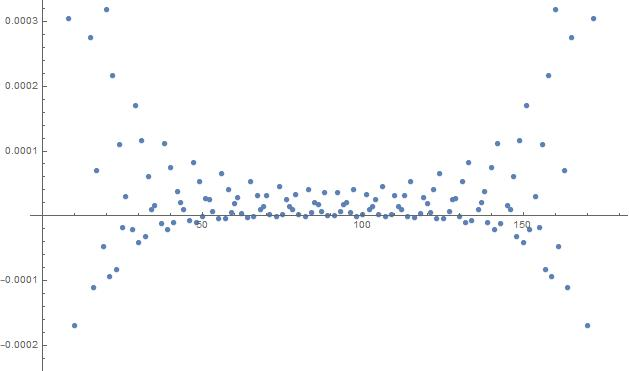
\includegraphics[scale=0.45]{Boundary.jpg}
\caption{Numerical value of $u$ at boundary points}
\end{figure}

\par To summarize the performance of BEM, we can conclude boundary element solution have a highly accuracy at interior points and more constant elements indicate a higher accuracy of the numerical solution. Although at boundary points, boundary element solution is not well-defined, we can still approximate the value at boundary points by taking the value at an interior point which is fairly close to the boundary point. 

\par In real problems, the boundaries are often complex and irregular, where the analytical solution is often difficult to obtain. But the boundary element method are still valid for those problem and could hold a fairly high accuracy. Therefore, boundary element method is a quite general method to solve boundary value problems and is widely used in the engineering field. 
\section{Boundary Element Method Using Green Function} 
Now that we know the basic BEM principle and have successfully solved a simple boundary value problem with BEM, but can we explore more about BEM? As we all known, the Green function is a special kind of fundamental solution with homogeneous boundary conditions, so what would boundary element solution be if we substitute the Green function instead of ordinary fundamental solution? In this section, we will study with boundary element solution using Green function and based on that solve the pre-defined Dirichlet problem.
\subsection{Boundary Element Solution Using Green Function} 
\par According to previous section, one of the fundamental solutions of  the operator $-\Delta$ is
\begin{equation*}
E(x;\xi) = - \frac{1}{2\pi}\ln|x -\xi| \ \ [1]
\end{equation*}
Then, applying methods of images, it is easy to find the green function of Dirichlet problem governed by $-\Delta$ on the upper half-plane as
\begin{equation}
g(x;\xi) = E(x;\xi) - E(x;\xi^*) \ \ [1]
\end{equation}  
where $\xi^* = (\xi_1,-\xi_2)$ supposing $\xi = (\xi_1,\xi_2)$ [1]. 

\par Thus, for the domain $\Omega$ defined in Eq. (1), we suppose $\partial \Omega = L \cup C$ where $L$ denotes the bottom line of the semi circle, $x_2 = 0$, and $C$ denotes the upper curve of the semi-circle, $\sqrt{x_1^2 + x_2^2} = 1$[1]. Since $g(x;\xi)|_{x \in L} = 0$ and $\frac{\partial g(x;\xi)}{\partial n}|_{x \in L} = 0$, substituting the Green function into the boundary integral solution, we can get 
\begin{equation}
\lambda(\xi)u(\xi) = \int_{C} [u(x)\frac{\partial g(x_;\xi)}{\partial n} - g(x;\xi) \frac{\partial u(x)}{\partial n}] ds \ \ [1] 
\end{equation}
where $\lambda (\xi)$ is defined as
\begin{equation}
\lambda(\xi) = \left\{
\begin{aligned}
&0 &{\rm if} \xi \in L \cup \bar{\Omega}^c\\
&\frac{1}{2} &{\rm if} \xi \in C\\
&1 &{\rm if} \xi \in \Omega \cap \xi \notin C\\
\end{aligned} 
\right. \ \ [1]
\end{equation}


\par As usual, to obtain the boundary element solution, we will divide $C$ into $N$ small line segments which can be roughly illustrated as the figure below.

\begin{figure}[H]
\centering
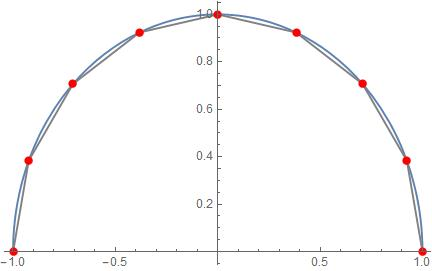
\includegraphics[scale=0.6]{segments2.jpg}
\caption{Rough Idea to Divide Boundar $C$}
\end{figure}
\noindent Thus, the boundary $C$ can be approximately equal to the combination of all the line segments. That is
\begin{equation}
C \approx C^1 \cup C^2 \cup \cdots \cup C^{N-1} \cup C^N \ \ [2]
\end{equation} 
where $C^k$ represent each line segment. 

\par Also, as before, assuming that the value of $u$ and $\frac{\partial u}{\partial n}$ on each line segment is constant, we use the both values at the midpoint of each line segments as approximations to the real values. That is 
\begin{equation}
\begin{aligned}
&u \approx \bar{u}^k & \frac{\partial u}{\partial n} \approx \bar{p}^k \ {\rm for }\ (x_1,x_2) \in C^k (k = 1,2,\cdots, N) 
\end{aligned} \ \ [2]
\end{equation}
where $\bar{u}^k$ and $\bar{p}^k$ are the values of $u$ and $\frac{\partial u}{\partial n}$ at the midpoint of $C^k$ [2].
\par Then, it is easy for us to derive that
\begin{equation}
\lambda(\xi) u(\xi) \approx  \sum_{k = 1}^{N} (\bar{u}^{k}\int_{C^k} \frac{\partial g(\cdot;\xi)}{\partial n}ds  - \bar{p}^k\int_{C^k} g(\cdot;\xi)ds )  \ \ [1]
\end{equation}
where 
\begin{equation}
\begin{aligned}
&\int_{C^k} \frac{\partial g(\cdot;\xi)}{\partial n} ds= F_1^k(\xi) - F_1^k(\xi^*)\\
&\int_{C^k} g(\cdot;\xi) ds = F_2^k(\xi) - F_2^k(\xi^*)
\end{aligned} \ \ [1]
\end{equation} 
As before, we can also find $N$ unknown parameters. 

\par Thus, for the specific problem, Dirichlet Problem with Laplace operator on the half-disk, we rewrite our previous boundary element solution by changing the ordinary fundamental solution with green function of upper half plane. Then, to make the solution to this problem more intuitive, we plot the  numerical solution with $120$ constant elements in 3D-plane as shown in the figure 8.

\begin{figure}[H]
\centering
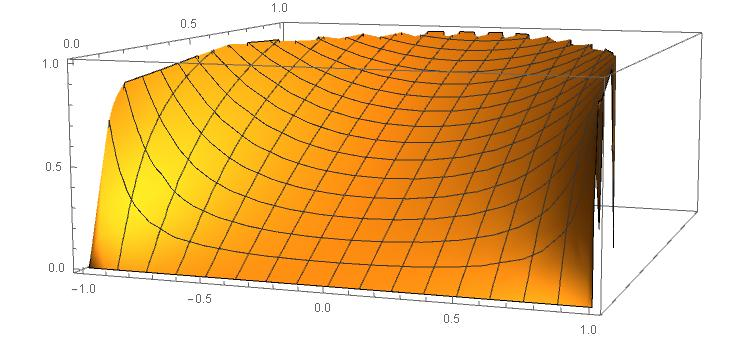
\includegraphics[scale=0.46]{BEM2.jpg}
\caption{Boundary element Solution using Green function to pre-defined Dirichlet Problem}
\end{figure}


\subsection{Comparison with Analytic Solution}
Comparing the plot of modified boundary element solution (figure 8) with the plot of analytic solution (figure 2), still, both plots are quite similar with each other at interior points and the plot of boundary element solution using Green function at the boundary is not as smooth as the plot of analytic solution. Then, to provide more evidence to support our statement drawing from the visual observation, we will compare these two solutions into details.  

Similarly as before, in the table 3, the value of $u$ given by boundary element solution using Green function (with $60$ and $120$ constant elements) at input interior points are compared with exact value. From the table, we can see that both boundary element solutions give good approximations to the exact value $u$ at given points. And we also notice that the one with a larger number of constant elements give a more accurate approximation. However, it should be mentioned that when applying boundary element solution using Green function, the differences of accuracies of two numerical solutions with different constant elements is not as large as those of previous numerical solutions without using Green function. Thus, we guess that with equal constant elements, BEM using Green function is more accurate than the previous one without using Green function. Without going into too much detail here, I will make a detailed comparison of the two methods in the next section.
\begin{table}[H]
\centering
\begin{tabular}{@{}cccc@{}}
\toprule
   $(\xi_1,\xi_2)$         & 60 Elements & 120 Elements & Exact    \\ \midrule
(0.10,0.20) & 0.253793    & 0.253729     & 0.253707 \\
(0.10,0.30) & 0.374455     & 0.374364      & 0.374334 \\
(0.10,0.40) & 0.488432     & 0.488321      & 0.488284 \\
(0.50,0.20) & 0.326824     & 0.326673      & 0.326623 \\
(0.50,0.30) & 0.469954     & 0.469769      & 0.469708 \\
(0.50,0.40) & 0.595719     & 0.595523      & 0.595458 \\
(0.90,0.20) & 0.772824     & 0.771899      & 0.771599 \\
(0.90,0.30) & 0.895567     & 0.895035      & 0.894863 \\
(0.90,0.40) & 0.976611     & 0.976256      & 0.976138 \\ \bottomrule
\end{tabular}
\caption{Comparing numerical value with exact value of $u$ at given points}
\label{tab:my-table}
\end{table}

\par Then, we also examine the accuracy of numerical value given by the boundary element solution using Green function with $80$ constant elements at the interior point $(0.1,a)$ as $a$ approaching 1. The results are show in the following table.
\begin{table}[H]
\centering
\begin{tabular}{@{}cccccc@{}}
\toprule
Error       & 0.95       & 0.96        & 0.97        & 0.98        & 0.99         \\ \midrule
80 Elements & 0.000104368 & 0.000104222 & 0.000104274 & 0.000105507 & 0.000112669\\ \bottomrule
\end{tabular}
\caption{Errors of numerical solution with $80$ constant elements}
\label{tab:my-table}
\end{table}
\par From the table 4, it is clear that as the interior point getting close to the boundary, error will also get large. Although the error at point $(0.1, 0.96)$ is a bit smaller than that at point $(0.1,0.95)$, the overall trend is still on the rise. 

\par We are also interested in how it performs at the boundary, therefore, we plot the value of $u$ given by modified boundary element solution at some points on the boundary and the plot is shown in the figure below. \begin{figure}[H]
\centering
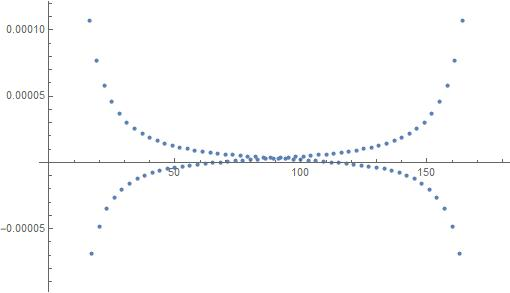
\includegraphics[scale=0.53]{Boundary2.jpg}
\caption{$u$ Given by Modified Boundary Element Solution at Some Boundary Points}
\end{figure}

\par Still, we can see from the graph, the value $u$ given by boundary element solution using Green function on the boundary points is undefined. 

\par Now, we have compared both boundary element solutions with the analytic solution. Both of them have a good accuracy and almost behaves in a same way, which is under our expectation because Green function is just one special fundamental solution and all the features that original boundary element solution holds should also be hold for the boundary element solution using Green function.  

\subsection{Comparison with Original Boundary Element Solution}
How does the boundary element solution using Green function perform compared with original boundary element solution. Based on the previous data, we guess that the one using Green function should have better accuracy than the one without using green function. Therefore, to prove our hypothesis, we compared the accuracy of both boundary element solutions with equal constant elements $120$ at some given interior points. The results are given in the following table. 

\begin{table}[H]
\centering
\begin{tabular}{@{}cccccc@{}}
\toprule
Error                  & (0.10,0.85)  & (0.10,0.88)   & (0.10,0.90)   & (0.10,0.93)  & (0.10,0.95)  \\ \midrule
With Green Fun.  & $4.68 \times 10^{-5}$ &$4.67 \times 10^{-5}$, & $4.66 \times 10^{-5}$, & $4.64 \times 10^{-5}$ & $4.63 \times 10^{-5}$ \\
Original & $9.90 \times 10^{-5}$ & $1.00 \times 10^{-4}$  & $1.01 \times 10^{-4}$   & $1.02  \times 10^{-4}$ & $1.02 \times 10^{-4}$  \\ \bottomrule
\end{tabular}
\caption{Comparison of errors of BEM using Green function and original BEM}
\label{tab:my-table}
\end{table}

From the above table, it is clear that with the same number of constant elements, the boundary element solution using Green function gives lower errors. Thus, we can conclude that at interior points, the boundary element solution using Green function gives a better approximation compared with original boundary element solution. 

\section{Boundary Element Solution With Mixed Boundary Conditions}
So far, we only focused on the Dirichlet problem which is simple and easy to calculate, but we know BEM can also be applied to complex BVP with even mixed boundary conditions like the mixture of Neumann condition and Dirichlet condition. Thus, in this section, we will investigate further on the performance of BEM when applied to mixed boundary value problem.

\subsection{Mixed Boundary Value Problem for the Laplace Equation On The Half-disk}
To study the BVP with mixed conditions, we will modified the original Dirichlet problem into mixed boundary value problem. That is
\begin{equation}
\Omega = \{ (x_1,x_2) \in R^2: x_1^2 + x_2^2 < 1, x_2 > 0 \}
\end{equation}

\par We set
\begin{align}
&- \Delta u = 0 \ {\rm on}\   \Omega & \begin{aligned}
&u(x_1,x_2)|_{x_1^2 + x_2^2} = 1 \\ &\frac{\partial u(x_1,0)}{\partial n} = -1 \ {\rm for} \ -1 < x_1 < 1
\end{aligned}
\end{align} 

\par In the following sections, we will focus on the newly defined problem to study the performance of BEM when solving mixed boundary value problem.

\subsection{Boundary Element Solution to Mixed Boundary Value Problem}
Similarly as before, we use Mathematica to obtain the boundary element solution (with $120$ constant elements) to the mixed boundary value problem (detailed code can be found in \textbf{Appendix}). And we plot our solution in the three-dimensional plane  as shown in the figure 10 below,.

\begin{figure}[H]
\centering
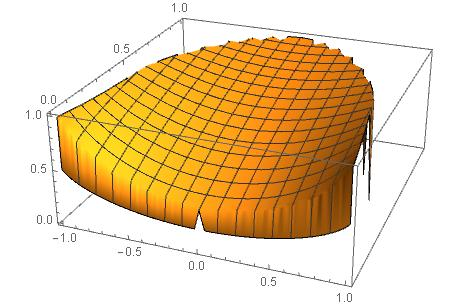
\includegraphics[scale=0.55]{BEM3.jpg}
\caption{Boundary Element Solution to Mixed Boundary Value Problem}
\end{figure}

Also, to make a comparison, we use the finite element methods built inside Mathematica to obtain another numerical solution which holds sufficient high accuracy and can be approximately considered as the real solution to this problem. The plot of the numerical solution is given below.

\begin{figure}[H]
\centering
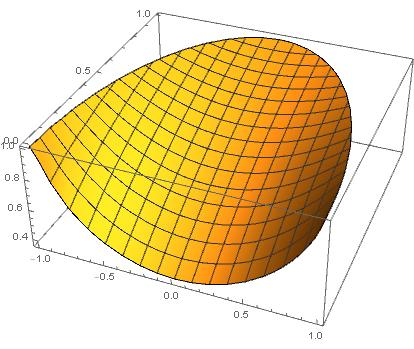
\includegraphics[scale=0.55]{analytic2.jpg}
\caption{Approximate Real solution to Mixed Boundary Value Problem}
\end{figure}

\par Comparing the two plots, although their shapes look similar, it is hard for us to see if the boundary element method provides an accurate solution to the mixed boundary element problem. Therefore, we should look deeply into data and compare these two solutions into details. 

\par In the table below, the numerical value of $u$ of the boundary element solution with $60$ and $120$ constant elements at some given interior points $(\xi_1,\xi_2)$ is compared with numerical value of $u$ of finite element solution which can be approximately considered as the real value of $u$ at those points. 

\begin{table}[H]
\centering
\begin{tabular}{@{}cccc@{}}
\toprule
    $(\xi_1,\xi_2)$        & 60 Element & 120 Element & Approximate Exact value \\ \midrule
(0.10,0.20) & 0.551203   & 0.550764   & 0.551841    \\
(0.10,0.30) & 0.630278   & 0.629848   & 0.630815    \\
(0.10,0.40) & 0.701632   & 0.701225   & 0.702062    \\
(0.50,0.20) & 0.653107   & 0.652429   & 0.652624    \\
(0.50,0.30) & 0.725203   & 0.724614   & 0.724802    \\
(0.50,0.40) & 0.788329   & 0.787831   & 0.788019    \\
(0.90,0.20) & 0.924841   & 0.924011   & 0.923646    \\
(0.90,0.30) & 0.959895   & 0.959372   & 0.959226    \\
(0.90,0.40) & 0.990241   & 0.989907   & 0.989775    \\ \bottomrule
\end{tabular}
\caption{Comparing numerical value with approximate exact value}
\label{tab:my-table}
\end{table} 

\par From the table above, we can see that as the number of constant elements increases, the accuracy of our boundary element solution also increases. And both two boundary element solutions gives a good approximation to the real solution of this problem. 

\par As before, we then examine the accuracy of value of $u$ given by boundary element solution as the points getting closer to the boundary. Here, we use the boundary element solution with $120$ constant elements and examine the accuracy at interior point $(0.1,a)$ where $a$ will approach $1$ gradually. The observed results are listed in the following table. 

\begin{table}[H]
\centering
\begin{tabular}{@{}cccccc@{}}
\toprule
Error       & 0.95        & 0.96        & 0.97        & 0.98        & 0.99       \\ \midrule
120 Elements & $3.74 \times 10^{-6}$ & $7.97 \times 10^{-6}$ &  $2.07 \times 10^{-5}$ &  $2.57 \times 10^{-5}$ &  $3.87 \times 10^{-5}$ \\ \bottomrule
\end{tabular}
\caption{Errors of numerical solution with $120$ constant elements}
\label{tab:my-table}
\end{table}

\par From the table above, it is clear that as the points approaching to the boundary, the errors get larger and larger. 

\par However, it should be still noticed that here we use the numerical solution obtained by finite element method as the real solution to the problem, although it holds a fairly high accuracy, it can not really replace the real solution to the problem. Therefore, we cannot conclude any reliable statement from the data, but roughly, we can still say that boundary element solution should be very close to the real solution to the problem. 

\par In terms of above results, we can summarize that BEM is still valid for those complex mixed boundary value problems and the numerical solutions of mixed boundary value problems still behaves in the same way as those of simple Dirichlet problem. 
\section{Conclusion and Discussion}

\subsection{Conclusion}
In this paper, we first analyze the internal principle and performance of BEM in detail by applying BEM to a simple Dirichlet problem. Then, we discuss the modified boundary element solution using Green function, which has a better performance than the previous one without using Green function. Finally, we change our pre-defined Dirichlet problem to mixed boundary value problem and try to use BEM to solve it which turns out to be valid and could give a fairly accurate numerical solution to the problem. Although during the analysis we found the numerical solution given by BEM is not well-defined at the boundary points, we can still take the value of nearby points as a proper approximation to the real value at the boundary. 
\par Thus, it could be concluded that BEM is a general method that can solve most boundary problems.

\subsection{Further Discussion}

\par The part of the article that I wanted to explore in detail is over, however, there are a few things more worth noting about BEM. 

\par As a numerical method, compared with the finite element method, the boundary element method has many excellent characteristics. Instead of divide the continuum domain into many small elements, the boundary element method only needs to divide the boundary into a finite number of line segments which could turn a high-dimensional problem into a lower-dimensional problem. Therefore, BEM has greatly reduced the computation of solve a boundary value problem and highly improved the accuracy of the numerical solution. 

\par However, BEM also has a big disadvantage, which is that BEM requires the corresponding green's function with an equation[3]. Because the boundary element method relates boundary conditions and internal unknowns through green's function, it is only applicable equations where green's function is easy to know[3]. Although there have been various ways to loosen the restrictions in recent times, this has fundamentally restricted the application of boundary element method to other problems such as hyperbolic equations[3].

\par Nevertheless, because of its simplicity and accuracy, BEM is still widely used in many fields.
\section{Works Cited}
\begin{itemize}
\item[{[}1{]}]H. Hohberger. ``vv557 video slides.pdf”. UMJI-SJTU, Shanghai. [Online; accessed 2-May-2020].
\item[{[}2{]}]
ANG, W. T. \textit{A Beginner’s Course in Boundary Element Methods}. Universal Publishers, Boca Raton, USA, 2007.
\item[{[}3{]}]
``Boundary element method," Wikipedia, 12-Apr-2020. [Online]. Available: \url{https://en.wikipedia.org/wiki/Boundary_element_method}. [Accessed: 02-May-2020].
\end{itemize}

\section{Appendix}
The detailed code are attached here.

\end{document}




